\documentclass[11pt,a4paper]{article}
\usepackage[T1]{fontenc}
\usepackage[utf8]{inputenc}
\usepackage[sc]{mathpazo}
\linespread{1.05}
\usepackage[a4paper,margin=2.5cm]{geometry}
\usepackage{amsmath,amssymb}
\usepackage{graphicx}
\usepackage{booktabs}
\usepackage{float}
\usepackage{enumitem}
\usepackage{microtype}
\usepackage[font=small,labelfont=bf,labelsep=period]{caption}
\usepackage{xcolor}
\definecolor{linkblue}{HTML}{1F4E9A}
\usepackage[colorlinks=true,linkcolor=linkblue,citecolor=linkblue,urlcolor=linkblue]{hyperref}
\hypersetup{pdftitle={Data center load on the U.S. grid},pdfauthor={Sahil}}
\setlist{itemsep=2pt,topsep=4pt}
\graphicspath{{figures/}}

\begin{document}

\begin{center}
{\LARGE\bfseries Data center load on the U.S.\ grid: evidence from hourly demand in PJM zones, and its carbon cost at the margin\par}
\vspace{1.1em}
{\large Sahil\par}
\vspace{0.3em}
{\small Whiting School of Engineering, Johns Hopkins University, Baltimore, MD, USA\par}
{\small\texttt{sfnu1@jh.edu}\par}
\vspace{0.8em}
{\small November 2026 \quad$\cdot$\quad Data through <<END>>, results generated <<RUN>>\par}
\end{center}

\vspace{0.6em}
\begin{center}\textbf{Abstract}\end{center}
\begin{quote}\small
Has the build-out of data centers since 2023 left a measurable mark on U.S.\ electricity demand, and what does serving it emit? This report uses <<RECORDS>> million hourly records from EIA Form~930, covering <<NR>> balancing authorities and <<NZ>> load zones of the PJM Interconnection, from <<START>> to <<END>>. Two zones separate from the rest. In the AEP zone (Ohio and Appalachia), yearly demand growth moved from <<AEP_B>>\% to <<AEP_A>>\%. A synthetic control that tracked the zone within <<A_RMSPE>>\% before 2023 is now <<A_GAP>>\% below it, a gap of <<A_MW>>~MW that ranks <<A_RANK>> zones in placebo tests. The Dominion zone (Virginia) is <<D_GAP>>\% above its control, but that divergence predates 2023; its speed-up beyond its earlier trend is <<DA_MW>>~MW and is not statistically conclusive. Structural break tests date the change to <<BR_A>> in AEP and <<BR_D>> in Dominion. In PJM, one more MWh of demand adds <<MEF>>~t of CO$_2$, <<MVA>>\% more than the average MWh. Serving the load that is new since 2023 emits about <<N_MT>>~Mt of CO$_2$ a year. Demand is observed by zone, not by customer, so attribution to data centers is circumstantial.
\end{quote}
\noindent{\small\textbf{Keywords:} electricity demand; data centers; synthetic control; structural break; marginal emissions; PJM; EIA-930}

\section{Introduction}

Utilities and grid operators have reported sharp increases in requests to connect large data centers, and forecasts of U.S.\ electricity demand have been revised upward after more than a decade of flat load. Forecasts and interconnection queues describe intentions. This report asks what has already happened in metered demand, using only public data, and puts three questions to it:
\begin{enumerate}[label=(\roman*)]
\item Where, and by how much, has demand departed from its earlier path?
\item When did the departure begin?
\item What does the additional demand emit, given which plants respond to it?
\end{enumerate}

PJM is the natural place to look. It is the largest U.S.\ grid operator, it contains Northern Virginia, the largest data center market in the world, and it publishes hourly demand for each of its utility zones. Zones inside one market share weather systems, fuel prices and a regional economy, which makes them usable as comparisons for one another.

\paragraph{Related work.} Several 2026 studies ask what data centers do to prices, with conflicting answers. An EPRI study finds that data center growth lowered average retail rates \cite{epri2026}; Meeks et al.\ find that data center entry raised them, most at investor-owned utilities \cite{meeks2026}; Rana et al.\ apply synthetic control to retail prices \cite{rana2026}; and Kay et al.\ use a dispatch model to attribute a 3 to 5\% rise in wholesale prices to existing data centers \cite{kay2026}. Muller prices the air pollution and greenhouse gas damages \cite{muller2026}. These papers start from data center capacity databases or dispatch models. This report starts from the other end, with metered zonal demand, and asks how much load has measurably arrived. It is closest in spirit to PJM's own forecast accuracy report \cite{pjmaccuracy}, which uses internal data.

\paragraph{Contributions.}
\begin{enumerate}[label=(\roman*)]
\item A zone-level comparison of demand growth before and after 2023 across all <<NZ>> usable PJM zones (Section~\ref{sec:zones}).
\item Synthetic control estimates for the two zones that stand out, with placebo inference, leave-one-out refits and a placebo start date (Section~\ref{sec:scm}).
\item Structural break dates for each zone's share of PJM demand (Section~\ref{sec:timing}).
\item Marginal emission factors for ten grid regions, and the emissions implied by the additional load (Sections~\ref{sec:mef} and~\ref{sec:emissions}).
\item A pre-specified follow-up on whether forecast load has arrived, with a first feasibility result (Section~\ref{sec:next}).
\item A reproducible pipeline: every number, table and figure in this report is regenerated from the public data by one command (Section~\ref{sec:repro}).
\end{enumerate}

\section{Data}

\subsection{Source}
All data comes from the U.S.\ Energy Information Administration's Form EIA-930, the Hourly Electric Grid Monitor \cite{eia930}, downloaded as six-month bulk files. Two tables are used: the balance table (hourly demand, net generation and generation by energy source for each balancing authority) and the subregion table (hourly demand for zones within the larger authorities). The sample runs from <<START>> to <<END>>. Ten balancing authorities are kept: PJM, ERCOT, MISO, SPP, NYISO, ISO-NE, CAISO, Southern Company, TVA and Duke Energy Carolinas. EIA's anomaly-adjusted columns are used where they exist.

\subsection{Cleaning}
The feed contains occasional reporting errors, including zeros and values several orders of magnitude too large. Hourly demand is cleaned in three steps. Values at or below zero are removed. Values more than 2.5 times, or less than 0.4 times, the median of the surrounding week (a centered 169-hour window) are removed. Gaps of up to six hours are filled by linear interpolation. A month is used only if at least 90\% of its hours are present. In PJM zones the filter removes well under 0.01\% of hours, except in the small Rockland zone, which is dropped for incomplete coverage. That leaves <<NZ>> zones.

\subsection{Emissions}
EIA-930 does not report emissions. Hourly CO$_2$ for each region is estimated as generation from coal, natural gas and petroleum multiplied by a fuel-specific factor taken from EIA's 2023 national totals of emissions and generation \cite{eiafaq}: <<EF_COAL>>~t/MWh for coal, <<EF_GAS>> for gas and <<EF_OIL>> for petroleum. All other sources are counted as zero. Section~\ref{sec:limits} discusses what this misses.

\section{Methods}

\subsection{Change in growth}\label{sec:m-growth}
For each zone and region, let $y_t$ be monthly mean demand, or the monthly 5th-percentile hour as a measure of baseload. I estimate
\begin{equation}
\log y_t = \alpha_{m(t)} + \beta_1 \tau_t + \beta_2 \max(\tau_t, 0) + \varepsilon_t ,
\label{eq:growth}
\end{equation}
where $\alpha_m$ are month-of-year effects and $\tau_t$ is time in years measured from January 2023. Yearly growth is $e^{\beta_1}-1$ before and $e^{\beta_1+\beta_2}-1$ after; the test of $\beta_2 = 0$ asks whether growth changed. Standard errors are Newey--West \cite{neweywest} with six lags. January 2023 is the first full month after the public release of ChatGPT and is fixed in advance for every unit.

\subsection{Synthetic control}\label{sec:m-scm}
For a zone of interest (unit 1), the outcome $y_{jt}$ is log monthly demand in zone $j$ measured against that zone's own 2019--22 mean, which removes level differences between zones \cite{doudchenko}. Weights over the $J$ comparison zones solve
\begin{equation}
\hat{w} = \arg\min_{w} \sum_{t < T_0} \Bigl( y_{1t} - \sum_{j=2}^{J+1} w_j\, y_{jt} \Bigr)^{2}
\quad \text{subject to} \quad w_j \ge 0,\ \ \sum_j w_j = 1 ,
\label{eq:scm}
\end{equation}
with $T_0$ = January 2023, and the estimated effect in month $t$ is $\hat{\delta}_t = y_{1t} - \sum_j \hat{w}_j y_{jt}$ \cite{adh2010,abadie2021}. Because the comparison zones experience the same weather systems, no temperature model is needed. I report the average of $\hat\delta_t$ over the latest 12 months, converted to megawatts.

Two versions are estimated. The \emph{levels} version is Equation~\eqref{eq:scm} as written. The \emph{acceleration} version first removes each zone's own pre-2023 linear trend, extended forward, so the gap measures only growth beyond what the zone was already doing. The second is the appropriate estimand when a zone was diverging before the period of interest.

Inference follows \cite{adh2010}. Each comparison zone is treated in turn as if it were the zone of interest, and the ratio of root mean squared prediction error (RMSPE) after 2023 to before is computed for all. The $p$-value is the rank of the true zone's ratio. With <<ND>> comparison zones the smallest attainable $p$-value is <<MINP>>. I also refit leaving out each comparison zone that carries weight, and run a placebo in time that uses only pre-2023 data and pretends the build-out began in January 2021.

Dominion was designated as the zone of interest before any estimation. AEP was not: it emerged as the fastest-accelerating zone in the comparison of Section~\ref{sec:m-growth}, and is reported as a second zone of interest with that caveat. Each is excluded from the other's comparison pool.

\subsection{Dating the change}
Each zone's share of total PJM demand cancels weather that is common across zones. To date a change in its trend I regress the monthly share $s_t$ on month effects and a linear trend, add a term for a kink at month $k$,
\begin{equation}
s_t = \alpha_{m(t)} + \gamma_1 t + \gamma_2 \max(t-k, 0) + \eta_t ,
\end{equation}
and take the largest $F$ statistic for $\gamma_2 = 0$ over all $k$ in the middle 70\% of the sample \cite{andrews}. The $p$-value is from a moving-block bootstrap \cite{kunsch} of the residuals of the no-break model, with blocks of six months and 999 draws, which preserves serial correlation.

\subsection{Marginal emissions}
Following \cite{hawkes,silerevans}, the marginal emission factor is the slope $b$ in a regression of hourly changes,
\begin{equation}
\Delta \mathrm{CO}_{2,t} = a + b\, \Delta D_t + c_1 \Delta W_t + c_2 \Delta S_t + u_t ,
\label{eq:mef}
\end{equation}
where $D$ is demand, $W$ wind output and $S$ solar output. Wind and solar do not respond to demand, but they ramp at the hours demand does; without the controls, a solar-rich region's morning ramp is mistaken for a clean response to load \cite{callaway}. Hours where either difference lies more than eight robust standard deviations from its median are dropped. Standard errors are heteroskedasticity- and autocorrelation-consistent with 24 lags. The model is estimated by region and year, and pooled with an interaction to test for a change after 2023. Replacing the dependent variable with the hourly change in each source's output gives the share of each source in the response to one more MWh.

\section{Results}

\subsection{Two zones accelerate}\label{sec:zones}
Of <<NZ>> PJM zones, two stand apart (Figure~\ref{fig:zones}, Table~\ref{tab:zones}). In the AEP zone, growth went from <<AEP_B>>\% a year in 2019--22 to <<AEP_A>>\% a year since, a change of <<AEP_C>> points. Dominion went from <<DOM_B>>\% to <<DOM_A>>\%, a change of <<DOM_C>> points. The largest change in any other zone is <<RESTMAX>> points. Most zones were shrinking slightly before 2023 and are growing slightly now, which is why a comparison group is needed: some of the turn is common to the whole grid.

\begin{figure}[H]
\centering
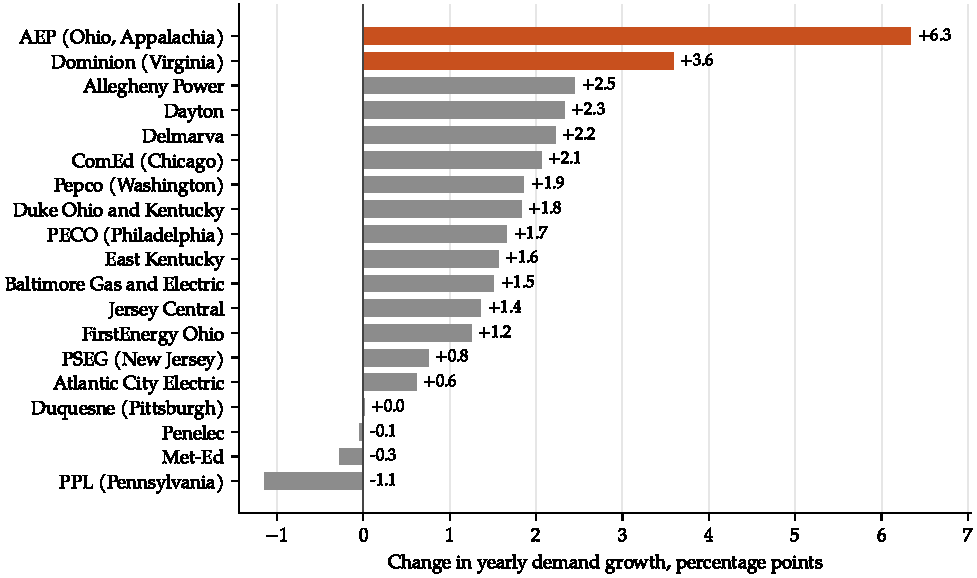
\includegraphics[width=0.88\linewidth]{fig1_zones.pdf}
\caption{Change in yearly demand growth, 2023 onward against 2019--22, by PJM zone.}\label{fig:zones}
\end{figure}

<<TAB_ZONES>>

\subsection{Synthetic control}\label{sec:scm}

\paragraph{AEP.} The synthetic control reproduces AEP's pre-2023 demand with an RMSPE of <<A_RMSPE>>\% (Figure~\ref{fig:aep}). Over <<W0>> to <<W1>>, AEP is <<A_GAP>>\% above it, or <<A_MW>>~MW on average (leave-one-out range <<A_LO>> to <<A_HI>>). Its post/pre error ratio ranks <<A_RANK>> ($p$ = <<A_P>>, the smallest attainable). The placebo start date gives a gap of <<A_PIT>>\%, as it should if nothing was happening before 2023. Removing AEP's own earlier trend leaves the estimate essentially unchanged, because that trend was flat (Table~\ref{tab:scm}).

\begin{figure}[H]
\centering
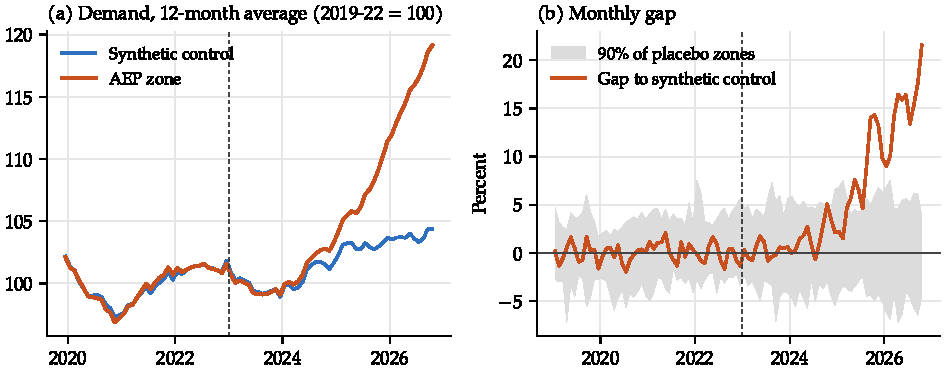
\includegraphics[width=\linewidth]{fig2_aep.pdf}
\caption{AEP zone against its synthetic control. The dashed line marks January 2023. The grey band in (b) contains 90\% of placebo zones.}\label{fig:aep}
\end{figure}

\paragraph{Dominion.} Dominion is <<D_GAP>>\% above its synthetic control (<<D_MW>>~MW), but the fit before 2023 is poor at <<D_RMSPE>>\%: no weighted average of other zones grew as fast as Dominion did even then (Figure~\ref{fig:dom}a). The placebo start date confirms it, with a gap of <<D_PIT>>\% using pre-2023 data alone. The levels estimate therefore measures Dominion's long-running divergence, not an effect dated to 2023. The acceleration version fits well before 2023 (<<DA_RMSPE>>\%) and finds a gap of <<DA_GAP>>\%, or <<DA_MW>>~MW, ranking <<DA_RANK>> ($p$ = <<DA_P>>). That is suggestive of a speed-up but does not meet a conventional threshold.

\begin{figure}[H]
\centering
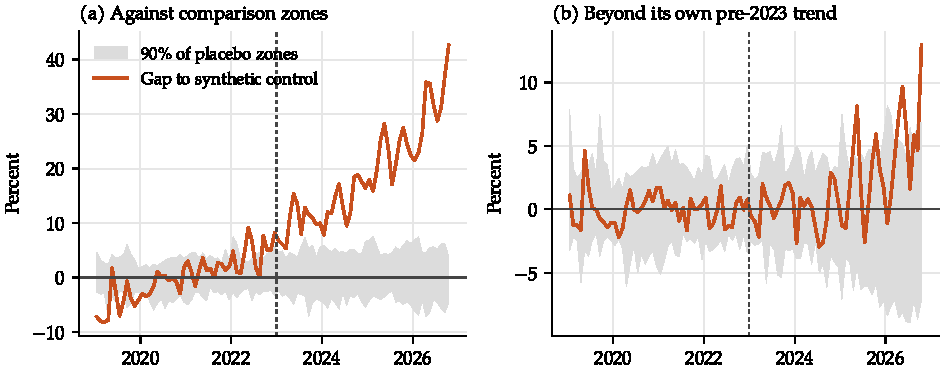
\includegraphics[width=\linewidth]{fig3_dominion.pdf}
\caption{Dominion zone: gap to its synthetic control under the two specifications.}\label{fig:dom}
\end{figure}

<<TAB_SCM>>
<<TAB_WEIGHTS>>

\subsection{Timing}\label{sec:timing}
Dominion's share of PJM demand rose from <<SH_D0>>\% to <<SH_D1>>\%, and AEP's from <<SH_A0>>\% to <<SH_A1>>\% (Figure~\ref{fig:share}). The break test dates the change in slope to <<BR_A>> for AEP (<<BR_AP>>) and <<BR_D>> for Dominion (<<BR_DP>>); see Table~\ref{tab:break}. Neither date was imposed. Both fall well after January 2023, which is what a construction-led increase would produce, since large facilities take a year or more to build and energize. It also means the January 2023 cut-off used elsewhere is conservative: it places some pre-surge months in the ``after'' period.

\begin{figure}[H]
\centering
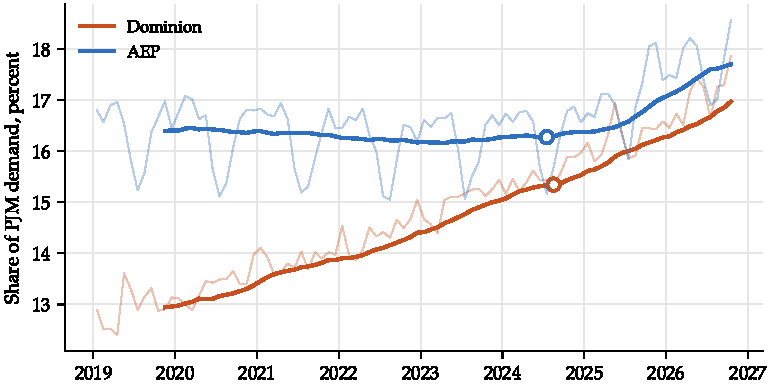
\includegraphics[width=0.85\linewidth]{fig4_share.pdf}
\caption{Share of PJM demand. Thin lines are monthly values, thick lines 12-month averages. Open circles mark estimated break dates.}\label{fig:share}
\end{figure}

<<TAB_BREAK>>

\subsection{Other regions}
Applying Equation~\eqref{eq:growth} to baseload in ten regions, growth increased significantly at the 5\% level in <<NSIG>> of <<NR>> (Figure~\ref{fig:regions}, Table~\ref{tab:regions}). The evidence is regional, not national. ERCOT has the fastest baseload growth of any region in both periods, so its increase is hard to separate from its own trend. These regional estimates have no comparison group and should be read as descriptive.

\begin{figure}[H]
\centering
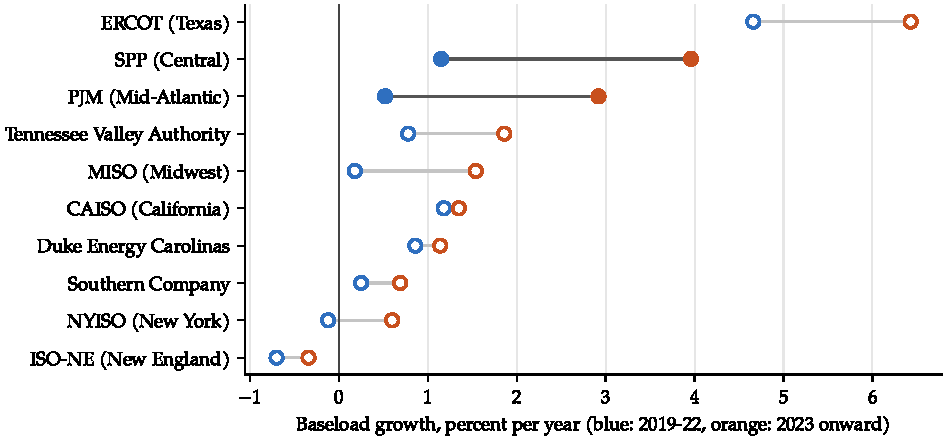
\includegraphics[width=0.88\linewidth]{fig5_regions.pdf}
\caption{Baseload growth before and after 2023 by grid region. Filled markers indicate a change significant at the 5\% level.}\label{fig:regions}
\end{figure}

<<TAB_REGIONS>>

\subsection{Marginal emissions}\label{sec:mef}
In PJM the marginal emission factor since 2023 is <<MEF>>~t/MWh (95\% interval <<MEF_LO>> to <<MEF_HI>>), down from <<MEF_PRE>> in 2019--22 (<<MEF_P>> for the change). Average intensity in the latest full year is <<AEF>> (Figure~\ref{fig:mef}a). The marginal MWh carries <<MVA>>\% more CO$_2$ than the average one because nuclear, which supplies about a third of PJM's energy, does not respond to demand. Since 2023, gas provides <<MX_GAS>>\% of the response to an extra MWh, coal <<MX_COAL>>\%, hydro and pumped storage <<MX_HYD>>\%, and imports <<MX_IMP>>\% (Figure~\ref{fig:mef}b). Table~\ref{tab:mef} gives the factors for all ten regions.

\begin{figure}[H]
\centering
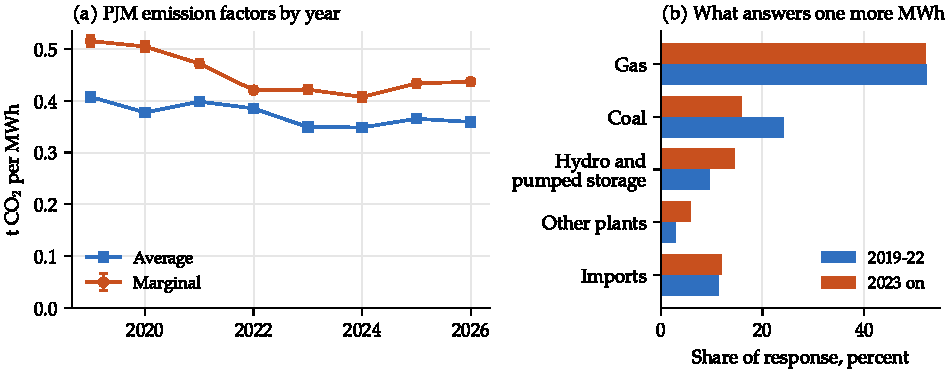
\includegraphics[width=\linewidth]{fig6_emissions.pdf}
\caption{PJM: (a) marginal and average emission factors by year, with 95\% intervals; the latest year is to date. (b) Share of each source in the response to one more MWh of demand.}\label{fig:mef}
\end{figure}

<<TAB_MEF>>

\subsection{Emissions from the additional load}\label{sec:emissions}
Summing the acceleration estimates for the two zones gives <<N_MW>>~MW of demand that is new since 2023, or <<N_TWH>>~TWh a year. At PJM's marginal factor that is <<N_MT>>~Mt of CO$_2$ a year, with a range of <<N_MT_LO>> to <<N_MT_HI>> from the leave-one-out refits and the interval on the marginal factor. Using the average factor would give <<N_MT_AVG>>~Mt. If all of Dominion's divergence from comparison zones is counted, including the part that predates 2023, the load is <<B_MW>>~MW and the emissions <<B_MT>>~Mt a year (Table~\ref{tab:emissions}).

<<TAB_EMISSIONS>>

\section{Robustness}
\begin{itemize}
\item \textbf{Comparison pool.} Leave-one-out refits move the AEP estimate between <<A_LO>> and <<A_HI>>~MW. No single comparison zone drives it.
\item \textbf{Pre-existing trends.} The placebo start date separates the two zones cleanly: <<A_PIT>>\% for AEP and <<D_PIT>>\% for Dominion. This is why Dominion's headline number uses the acceleration version.
\item \textbf{Contamination between zones.} Each zone of interest is removed from the other's comparison pool. Other zones may also host data centers, which would bias the estimates toward zero.
\item \textbf{Load shape.} Load factor (mean over peak demand) has risen in both zones and fallen in the rest of PJM, consistent with added round-the-clock load. Baseload shows the same acceleration as mean demand (Table~\ref{tab:zones}).
\item \textbf{Estimator checks.} On a synthetic grid with a planted 10\% a year effect and a planted marginal factor, the code recovers both within tolerance and finds nothing in zones with no planted effect. These tests run before every weekly refresh.
\end{itemize}

\section{Limitations}\label{sec:limits}
\begin{itemize}
\item \textbf{Attribution.} EIA-930 reports demand by zone. Factories, electrification and population growth also add load. The case for data centers rests on location, timing, the flatness of the added load and public reporting, not on direct observation. One external check is available: PJM reports that at the July 2025 peak, 68.1\% of its data center load was in the Dominion zone and 21.1\% in AEP \cite{pjmaccuracy}, the same two zones this analysis singles out.
\item \textbf{Selection of AEP.} AEP was identified from the data. Its $p$-value does not account for having searched across zones for the largest change.
\item \textbf{Coarse inference.} Placebo $p$-values cannot fall below <<MINP>> with this many zones.
\item \textbf{Emission factors.} One national factor per fuel ignores differences in plant efficiency. Marginal gas units are often less efficient than the fleet average, so the marginal factor here is more likely too low than too high.
\item \textbf{Regional boundary.} Emissions are counted within each balancing authority. Imports, about <<MX_IMP>>\% of PJM's marginal response, are not traced to their source.
\item \textbf{Short-run margin.} The marginal factor describes which existing plants respond hour to hour. It does not capture new plants built, or retirements delayed, because of sustained load growth.
\item \textbf{Behind-the-meter supply.} Data centers with on-site generation do not appear in zonal demand.
\end{itemize}

\section{Next step: did the forecast load arrive?}\label{sec:next}
PJM's capacity auctions clear against its load forecast, which has been revised sharply upward for data centers. Analysts argue that the forecasts are inflated by speculative requests \cite{gridstrategies}. The natural follow-up to this report is to test that against metered demand: compare each January forecast, by zone and horizon, with the load that was later metered, and compare zones whose forecasts carry a data center adjustment with zones whose forecasts do not.

A feasibility check has been run and nothing more; the result below is preliminary (22 November 2026). All eight PJM Load Forecast Reports from 2019 to 2026 can be retrieved. For calendar year 2025, one year ahead, realized zonal energy from EIA-930 differs from PJM's January 2025 forecast by a median of 1.5\% in absolute value across 19 zones, so the two sources are comparable. AEP came in 0.4\% below its forecast and Dominion 2.8\% above. At this short horizon the forecast load did arrive. The open question is the longer horizons that the auctions depend on, which can only be evaluated as more years accumulate. The hypotheses, outcome and sample rules for that study are written down in advance in a separate research plan, available on the project website.

\section{Reproducibility}\label{sec:repro}
The pipeline is a downloader, the analysis, a test suite and the script that builds this report. It needs no API key and runs in about two minutes on a standard GitHub Actions runner, which re-executes it every Monday. Random seeds are fixed. This report is regenerated by \texttt{report/build\_report.py} from the same results file the website reads, so the two cannot disagree. Code: \url{https://github.com/sahiljangra12/grid-data-centers}. Website: \url{https://sahiljangra12.github.io/grid-data-centers/}.

\begin{thebibliography}{99}\small
\bibitem{adh2010} Abadie, A., Diamond, A., and Hainmueller, J. (2010). Synthetic control methods for comparative case studies: Estimating the effect of California's tobacco control program. \emph{Journal of the American Statistical Association}, 105(490).
\bibitem{abadie2021} Abadie, A. (2021). Using synthetic controls: Feasibility, data requirements, and methodological aspects. \emph{Journal of Economic Literature}, 59(2).
\bibitem{andrews} Andrews, D.~W.~K. (1993). Tests for parameter instability and structural change with unknown change point. \emph{Econometrica}, 61(4).
\bibitem{callaway} Callaway, D.~S., Fowlie, M., and McCormick, G. (2018). Location, location, location: The variable value of renewable energy and demand-side efficiency resources. \emph{Journal of the Association of Environmental and Resource Economists}, 5(1).
\bibitem{doudchenko} Doudchenko, N., and Imbens, G.~W. (2016). Balancing, regression, difference-in-differences and synthetic control methods: A synthesis. NBER Working Paper 22791.
\bibitem{epri2026} EPRI (2026). Have data centers raised your electric bill? arXiv:2606.19777.
\bibitem{gridstrategies} Grid Strategies (2025). Power demand forecasts revised up: National load growth report.
\bibitem{hawkes} Hawkes, A.~D. (2010). Estimating marginal CO$_2$ emissions rates for national electricity systems. \emph{Energy Policy}, 38(10).
\bibitem{kay2026} Kay, O., Reaser, R., and Taylor, R. (2026). Processing power: The effect of data centers on wholesale electricity markets. Federal Reserve Bank of Dallas Working Paper 2606.
\bibitem{kunsch} K\"unsch, H.~R. (1989). The jackknife and the bootstrap for general stationary observations. \emph{Annals of Statistics}, 17(3).
\bibitem{meeks2026} Meeks, R., Pless, J., Qi, Z., and Wang, Z. (2026). Who pays for growth? Evidence from data centers and the grid. MIT CEEPR Working Paper.
\bibitem{muller2026} Muller, N.~Z. (2026). Measuring the impact of data centers in the United States economy: Monetary damage from air pollution and greenhouse gas emissions. NBER Working Paper 35100.
\bibitem{neweywest} Newey, W.~K., and West, K.~D. (1987). A simple, positive semi-definite, heteroskedasticity and autocorrelation consistent covariance matrix. \emph{Econometrica}, 55(3).
\bibitem{pjmaccuracy} PJM Interconnection (2026). 2026 PJM load forecast accuracy report.
\bibitem{rana2026} Rana, V., Kaps, C., and Netessine, S. (2026). The cost of intelligence: Impacts of AI data centers on US electricity prices. SSRN Working Paper.
\bibitem{silerevans} Siler-Evans, K., Azevedo, I.~L., and Morgan, M.~G. (2012). Marginal emissions factors for the U.S.\ electricity system. \emph{Environmental Science \& Technology}, 46(9).
\bibitem{eia930} U.S.\ Energy Information Administration. Form EIA-930, Hourly Electric Grid Monitor. \url{https://www.eia.gov/electricity/gridmonitor/}.
\bibitem{eiafaq} U.S.\ Energy Information Administration. How much carbon dioxide is produced per kilowatthour of U.S.\ electricity generation? \url{https://www.eia.gov/tools/faqs/faq.php?id=74}.
\end{thebibliography}

\end{document}
